\documentclass{article}

\usepackage{amssymb, amsmath, amsthm}
\usepackage[margin=1in]{geometry}
\usepackage{verbatim}
\usepackage{graphicx}
\usepackage{hyperref} % \url \href
\usepackage{docmute}
\usepackage[title]{appendix}

\newtheorem{definition}{Definition}
\newtheorem{theorem}{Theorem}
\newcommand{\heff}{\mathbb{H}^{\text{eff}}}
\newcommand{\pfrac}[2]{\frac{\partial #1}{\partial #2}}
\newcommand{\huptb}{\text{H}_0}
\newcommand{\order}[2]{#1^{(#2)}}
\newcommand{\statebra}[1]{\langle #1 |}
\newcommand{\stateket}[1]{| #1 \rangle}
\newcommand{\MO}{\textbf{MO}}
\newcommand{\AO}{\textbf{AO}}

\begin{document}

\title{Orbital Interactions in Chemistry}
\author{Wenhao Zhang}
\date{\today}
\maketitle

\tableofcontents

\documentclass{article}
\usepackage{amssymb, amsmath, amsthm}
\usepackage[margin=1in]{geometry}
\usepackage{verbatim}
\usepackage{graphicx}
\usepackage{hyperref} % \url \href
\usepackage{docmute}

\newtheorem{definition}{Definition}
\newtheorem{theorem}{Theorem}
\newcommand{\heff}{\mathbb{H}^{\text{eff}}}
\newcommand{\pfrac}[2]{\frac{\partial #1}{\partial #2}}

\newcommand{\MO}{\textbf{MO}}
\newcommand{\AO}{\textbf{AO}}

\newcommand{\huptb}{\text{H}_0}
\newcommand{\order}[2]{#1^{(#2)}}
\newcommand{\statebra}[1]{\langle #1 |}
\newcommand{\stateket}[1]{| #1 \rangle}

\begin{document}

\section{Solution to the Molecular Orbtials}
In this section, we write out explicitly the solution of the molecular orbitals. In the next section,
we will focus on the perturbation treatment. 
Let's write the 
\begin{align}
    &\mathbf{\chi} = \left( \begin{matrix}
        \chi_1& \chi_2& \chi_3& \cdots& \chi_m
    \end{matrix} \right) \\
    &\mathbf{C}_i = \left( \begin{matrix}
        C_{1i} \\ C_{2i} \\ \vdots \\ C_{mi}
    \end{matrix} \right)
\end{align}
so that the \MO wavefunction can be written as dot product:
\begin{equation}
    \psi_i = \mathbf{\chi}\cdot \mathbf{C}_i = \sum_{\mu} C_{\mu i} \chi_{\mu}
\end{equation}
\MO s satisfy the eigenequation 
\begin{gather}
    \text{H}^{MO} \stateket{\psi_i} = \varepsilon_i \stateket{\psi_i} \\ 
    \sum_{\mu} \statebra{\chi_{\nu}}\text{H}\stateket{\chi_{\mu}}\statebra{\chi_{\mu}} \psi_i \rangle  = \sum_{\mu'} \varepsilon_i \statebra{\chi_{\nu}} \chi_{\mu'} \rangle \statebra{\chi_{\mu'}} \psi_i \rangle \\ 
    \sum_{\mu} \text{H}_{\nu\mu} C_{\mu i} =  \varepsilon_i S_{\nu \mu'} C_{\mu' i} \\ 
    \text{H}^{AO} \mathbf{C}_i = \varepsilon_i \mathbf{S}^{AO} \mathbf{C}_i
\end{gather}
in matrix form, we have:
\begin{equation}
    \mathbf{C} = \left( \begin{matrix} \mathbf{C}_1 & \mathbf{C}_2 & \cdots & \mathbf{C}_m \end{matrix} \right) 
    = \left( \begin{matrix}
        C_{11} & \cdots & C_{1m} \\
        \vdots & & \vdots \\ 
        C_{m1} & \cdots & C_{mm}  
    \end{matrix}\right)
\end{equation}
so that we can discard the index $i$:
\begin{equation}
    \textbf{H}^{AO} \mathbf{C} = \varepsilon \mathbf{S}^{AO} \mathbf{C}
\end{equation}
which is similar to an ordinary eigenequation except that the Hamiltonian 
is in a set of basis that are not orthogonal. The normalization of $\mathbf{C}$
is given with respect to overlap matrix $S$:
\begin{equation}
    \statebra{ \psi_i } \psi_j \rangle = \left( \sum_{\mu} C_{\mu i} \statebra{\chi_{\mu}} \right)  \left( \sum_{\nu} C_{\nu i} \stateket{\chi_{\nu}} \right) = \sum_{\mu\nu} c_{\mu i} c_{\nu i} S_{\mu \nu} = \delta_{ij}
\end{equation}
with real coefficients $\mathbf{C}$


\section{Molecular Perturbation Theory}
Let's consider the effect of perturbation on the molecular orbitals and their energies. The 
treatment is similar to that of the ordinary perturbation theory except that the basis functions 
are no longer orthogonal when the perturbation is introduced. For example, the change in geometry
by bringing two structure fragment together necessary introduce change in overlap so that the 
original wavefunctions are no longer orthogonal. This can be compared to text book perturbation
theory in quantum mechanics where only perturbation in Hamiltonian are introduced. As an example, 
let's consider the case of bringing the isolated molecular fragments $A$ and $B$ together to 
form molecular $AB$. In the original system, suppose we already solved the molecular orbitals on
each fragment. We can write down the system as
$H^0 C^0 = S^0 C^0 \varepsilon^0$ where
\begin{align}
    C^0 &= \left( \begin{matrix} C_A^0 & \mathbf{0} \\ \mathbf{0} & C_B^0 \end{matrix} \right) &
    S^0 &= \left( \begin{matrix} S_A^0 & \mathbf{0} \\ \mathbf{0} & S_B^0 \end{matrix} \right) \\
    H^0 &= \left( \begin{matrix} H_A^0 & \mathbf{0} \\ \mathbf{0} & H_B^0 \end{matrix} \right) &
    \varepsilon^0 &= \left( \begin{matrix} \varepsilon_A^0 & \mathbf{0} \\ \mathbf{0} & \varepsilon_B^0 \end{matrix} \right) \\
\end{align}
This is the block diagonal form composed of solutions of the molecular orbital coefficients $C_A^0$ and $C_B^0$
for each isolated fragments. In the case of the solution, the Hamiltonian is diagonalized and 
the overlap matrix is simply identity matrix. 

Now, the molecular orbital coefficients solved on the perturbed Hamiltonian can be written as 
\begin{equation}
    \label{perturbation_coefficients}
    \stateket{\psi_i} = \sum_j T_{ji} \stateket{\psi^0_j}
\end{equation}
we write down the perturbation as:
\begin{align}
    H = H^0 + \delta H \\
    S = S^0 + \delta S
\end{align}
We have the secular equation:
\begin{equation}
    (H - \varepsilon_i S) C_i = \left[ (H^0 + \delta H) - \varepsilon_i (S^0 + \delta S) \right] C_i = 0
\end{equation}
Using equation \eqref{perturbation_coefficients} and the fact that $\stateket{\psi^0_j}$ diagonalize $S^0$ and $H^0$
\footnote{is the solution of the secular equation spontaneously diagonalize H and S?},
we have:
\begin{align}
    (\varepsilon^0 + \delta H) T_i = \varepsilon_i (1 + \delta S) T_i
\end{align} 
which we simplify to $(h - \varepsilon_i S) T_i = 0$, where:
\begin{align}
    h &= \order{h}{0} + \lambda \order{h}{1} \\ 
    s &= \order{s}{0} + \lambda \order{s}{1} \\ 
    \varepsilon_i &= \order{\varepsilon_i}{0} + \lambda \order{\varepsilon_i}{1} + \lambda^2 \order{\varepsilon_i}{2} + \cdots \\
    T_i &= \order{T_i}{0} + \lambda \order{T_i}{1} + \lambda^2 \order{T_i}{2} + \cdots \\ 
\end{align}
Substituting these quantity into $(h - \varepsilon_i S) T_i = 0$ and matching the order up to second order, we find:
\begin{align}
    \left[(\order{h}{0} - \order{\varepsilon_i}{0}\order{S}{0}) + \lambda (\order{h}{1} - \order{\varepsilon_i}{1} \order{S}{0} - \order{\varepsilon_i}{0} \order{S}{1}) - \lambda^2 (\order{\varepsilon_i}{2} \order{S}{0} + \order{\varepsilon_i}{1} \order{S}{1})\right] \\ 
    \times \left( \order{T_i}{0} + \lambda \order{T_i}{1} + \lambda^2 \order{T_i}{2} \right) = 0
\end{align}
The zeroth order simply is the unperturbed solution, to first order, writting $\order{T_i}{1} = \sum_{j} a_{ji} \order{T_j}{0}$, we have:
\begin{equation}
    \label{E:mop_firstorder}
    (\order{h}{1} - \order{\varepsilon_i}{1} \order{S}{0} - \order{\varepsilon_i}{0} \order{S}{1}) \order{T_i}{0} + (\order{h}{0} - \order{\varepsilon_i}{0}\order{S}{0}) \sum_{k} a_{ki} \order{T_k}{0} = 0
\end{equation}
We use the following relationship:
\begin{align}
    (\order{T_j}{0})^T \order{T_i}{0} &= \delta_{ij}  & &\\ 
    (\order{T_j}{0})^T \order{h}{1} \order{T_i}{0} &= \tilde{H}_{ij} & (\order{T_j}{0})^T \order{h}{0} \order{T_i}{0} &= \varepsilon_i \delta_{ij}\\ 
    (\order{T_j}{0})^T \order{S}{1} \order{T_i}{0} &= \tilde{S}_{ij} & (\order{T_j}{0})^T \order{S}{0} \order{T_i}{0} &= \delta_{ij}\\
\end{align}
we multiply equation \eqref{E:mop_firstorder} with $(\order{T_i}{0})^T$ on the left to obtain:
\begin{gather}
    ( \tilde{H}_{ii} - \order{\varepsilon_i}{1} - \order{\varepsilon_i}{0} \tilde{S}_{ii} ) + a_{ii} (\order{\varepsilon_i}{0} - \order{\varepsilon_i}{0}) = 0 \\ 
    \order{\varepsilon_i}{1} = \tilde{H}_{ii} - \order{\varepsilon_i}{0} \tilde{S}_{ii}
\end{gather}
multiply \eqref{E:mop_firstorder} with $(\order{T_j}{0})^T; (j\neq i)$ on the left, we obtain:
\begin{gather}
    ( \tilde{H}_{ij}- \order{\varepsilon_i}{0} \tilde{S}_{ij} ) + \sum_k \delta_{jk} a_{ki} (\order{\varepsilon_j}{0} - \order{\varepsilon_i}{0}) = 0 \\ 
    a_{ji}(j\neq i) = \frac{\tilde{H}_{ij}- \order{\varepsilon_i}{0} \tilde{S}_{ij}}{\order{\varepsilon_i}{0} - \order{\varepsilon_j}{0}}
\end{gather}
For second order, we have:
\begin{equation}
    (\order{h}{0} - \order{\varepsilon_i}{0}\order{S}{0}) \order{T_i}{2} + (\order{h}{1} - \order{\varepsilon_i}{1} \order{S}{0} - \order{\varepsilon_i}{0} \order{S}{1}) \order{T_i}{1} 
    - (\order{\varepsilon_i}{2} \order{S}{0} + \order{\varepsilon_i}{1} \order{S}{1}) \order{T_i}{0} = 0
\end{equation} 
using the results for the first order perturbation and multiplying $(\order{T_i}{0})^T$ or  $(\order{T_j}{0})^T; (j\neq i)$ on the left, we find the 
result:
\begin{align}
    \order{\varepsilon_i}{2} &= - \order{\varepsilon_i}{0} \tilde{S}_{ii} + \sum_{j\neq i} \frac{(\tilde{H}_{ij}- \order{\varepsilon_i}{0} \tilde{S}_{ij})^2}{\order{\varepsilon_i}{0} - \order{\varepsilon_j}{0}} \\ 
    b_{ji} (j\neq i) &= - \frac{(\tilde{H}_{ii}- \order{\varepsilon_i}{0}\tilde{S}_{ii} )\tilde{S}_{ij}}{\order{\varepsilon_i}{0} - \order{\varepsilon_j}{0}}
    + \sum_{k\neq i} \frac{(\tilde{H}_{ik}- \order{\varepsilon_i}{0} \tilde{S}_{ik})(\tilde{H}_{kj}- \order{\varepsilon_i}{0} \tilde{S}_{kj})}{(\order{\varepsilon_i}{0} - \order{\varepsilon_j}{0})(\order{\varepsilon_i}{0} - \order{\varepsilon_k}{0})}
\end{align}
so that $\order{T_i}{2} = \sum_j b_{ji} \order{T_j}{0}$.

Now, we note that the coefficient $a_{ii}$ and $b_{ii}$ are not yet obtained. They are given by the normalization condition as well as to the previous results, we have:
\begin{align}
    \order{T_{ii}}{1} &= - \frac{1}{2} \tilde{S}_{ii} \\ 
    \order{T_{ii}}{2} &= 
    - \sum_{j\neq i} \frac{(\tilde{H}_{ij} - \order{\varepsilon_i}{0}\tilde{S}_{ij})\tilde{S}_{ij}}{\order{\varepsilon_i}{0} - \order{\varepsilon_j}{0}}
    - \frac{1}{2} \sum_{j\neq i} \left(\frac{\tilde{H}_{ij} - \order{\varepsilon_i}{0}\tilde{S}_{ij}}{\order{\varepsilon_i}{0} - \order{\varepsilon_j}{0}} \right)^2
\end{align}

Finally, we obtain the complete result up to second order:
\begin{align}
    \varepsilon_i &= \order{\varepsilon_i}{0} + \underbrace{(\tilde{H}_{ii} - \order{\varepsilon_i}{0} \tilde{S}_{ii})}_{1^{th} order} 
    - \underbrace{\order{\varepsilon_i}{0} \tilde{S}_{ii} + \sum_{j\neq i} \frac{(\tilde{H}_{ij}- \order{\varepsilon_i}{0} \tilde{S}_{ij})^2}{\order{\varepsilon_i}{0} - \order{\varepsilon_j}{0}} }_{2^{nd} order}  \\ 
    T_{ii} &= 1 - \underbrace{\frac{1}{2} \tilde{S}_{ii}}_{1^{th} order} - \underbrace{\sum_{j\neq i} \frac{(\tilde{H}_{ij} - \order{\varepsilon_i}{0}\tilde{S}_{ij})\tilde{S}_{ij}}{\order{\varepsilon_i}{0} - \order{\varepsilon_j}{0}}
    - \frac{1}{2} \sum_{j\neq i} \left(\frac{\tilde{H}_{ij} - \order{\varepsilon_i}{0}\tilde{S}_{ij}}{\order{\varepsilon_i}{0} - \order{\varepsilon_j}{0}} \right)^2}_{2^{nd} order} \\ 
    T_{ji} &= \underbrace{\frac{\tilde{H}_{ij}- \order{\varepsilon_i}{0} \tilde{S}_{ij}}{\order{\varepsilon_i}{0} - \order{\varepsilon_j}{0}} }_{1^{th} order}
    - \underbrace{\frac{(\tilde{H}_{ii}- \order{\varepsilon_i}{0}\tilde{S}_{ii} )\tilde{S}_{ij}}{\order{\varepsilon_i}{0} - \order{\varepsilon_j}{0}}
    + \sum_{k\neq i} \frac{(\tilde{H}_{ik}- \order{\varepsilon_i}{0} \tilde{S}_{ik})(\tilde{H}_{kj}- \order{\varepsilon_i}{0} \tilde{S}_{kj})}{(\order{\varepsilon_i}{0} - \order{\varepsilon_j}{0})(\order{\varepsilon_i}{0} - \order{\varepsilon_k}{0})} }_{2^{nd} order}
\end{align}

Slight simplification can be given if we assume that $\delta H$ and $\delta S$ separately for the two fragments are zero:
\begin{align}
    \delta H = \left( \begin{matrix} \mathbf{0} & \delta H_{AB} \\ \delta H_{BA}  & \mathbf{0} \end{matrix} \right); \quad
    \delta S = \left( \begin{matrix} \mathbf{0} & \delta S_{AB} \\ \delta S_{BA}  & \mathbf{0} \end{matrix} \right)
\end{align}
in which case, the terms in the expansion like $(\tilde{H}_{ii} - \order{\varepsilon_i}{0} \tilde{S}_{ii})$ will be zero, and the summation 
are restricted with respect to the fragments where those states come from. 
The degenerate case can proceed similar to the non-degenerate theory, with the coefficients $T_{ji}^0$ no longer simply given by $\delta_{ji}$. 
We omit the degenerate treatment here.


\end{document}

\documentclass{article}
\usepackage{amssymb, amsmath, amsthm}
\usepackage[margin=1in]{geometry}
\usepackage{verbatim}
\usepackage{graphicx}
\usepackage{hyperref} % \url \href
\usepackage{docmute}

\newtheorem{definition}{Definition}
\newtheorem{theorem}{Theorem}
\newcommand{\heff}{\mathbb{H}^{\text{eff}}}
\newcommand{\pfrac}[2]{\frac{\partial #1}{\partial #2}}

\begin{document}

\section{Two-orbital solution}
We illustrate the application of the direct solution method using the two (atomic) orbital problem. Suppose the 
value of the parameters $H_{11} = \varepsilon_1^0$, $H_{22} = \varepsilon_2^0$, $H_{12}$ are known, as well as 
for the overlap: $S_{11} = S_{22} = 1$ and $S_{12}$. 
\begin{align}
    (\varepsilon_1^0 - \varepsilon_1) c_{11} + (H_{12} - \varepsilon_1 S_{12}) c_{21} &= 0 \\
    (H_{12} - \varepsilon_2 S_{12}) c_{12} + (\varepsilon_2^0 - \varepsilon_2) c_{22} &= 0 \\ 
    S_{ii} = c_{1i}^2 + c_{2i}^2 + 2 c_{1i} c_{2i} S_{12} &= 1
\end{align}
the energies can be solved by the determinant:
\begin{align}
    \left| \begin{matrix}
        \varepsilon_1^0 - \varepsilon_i & H_{12} - \varepsilon_i S_{12} \\
        H_{12} - \varepsilon_i S_{12} & \varepsilon_2^0 - \varepsilon_i
    \end{matrix} \right| &= 0 
\end{align}
therefore given by a second order equation:
\begin{equation}
    (\varepsilon_1^0 - \varepsilon_i)(\varepsilon_2^0 - \varepsilon_i) - (H_{12} - \varepsilon_i S_{12})^2 = 0
\end{equation}

\subsection{Degenerate case}
When $\varepsilon_1^0 = \varepsilon_2^0 = \varepsilon^0$, the solution for the energy can be found to be:
\begin{align}
    \varepsilon_1 = \frac{\varepsilon^0 + H_{12}}{1 + S_{12}} \approx \varepsilon^0 + (H_{12} - \varepsilon^0 S_{12}) - S_{12} (H_{12} - \varepsilon_i^0 S_{12}) \\
    \varepsilon_2 = \frac{\varepsilon^0 - H_{12}}{1 - S_{12}} \approx \varepsilon^0 - (H_{12} - \varepsilon^0 S_{12}) - S_{12} (H_{12} - \varepsilon_i^0 S_{12}) 
\end{align}
$S_{12} > 0$ and $H_{12} < 0$, we have thus $H_{12} - \varepsilon^0 S_{12} < 0$ so that $\varepsilon_1 < \varepsilon_2$, which are further shifted down by a small amount 
given by the second term.
The normalization coefficient can be solved using the secular relationship. We have:
\begin{equation}
    \frac{c_{21}}{c_{11}} = 1; \quad \frac{c_{22}}{c_{12}} = -1
\end{equation}
and the wave functios are:
\begin{align}
    \psi_1 = \frac{1}{\sqrt{2 + 2 S_{12}}} (\chi_1 + \chi_2) \\
    \psi_2 = \frac{1}{\sqrt{2 - 2 S_{12}}} (\chi_1 - \chi_2)
\end{align}

\subsection{Nondegenerate case}
Approximate results can be given for non-degenerate cases, with the solution for energies:
\begin{align}
    \varepsilon_1 \approx \varepsilon_1^0 + \frac{(H_{12} - \varepsilon_1^0 S_{12})^2}{\varepsilon_1^0 - \varepsilon_2^0} < \varepsilon_1^0 \\
    \varepsilon_2 \approx \varepsilon_2^0 + \frac{(H_{12} - \varepsilon_1^0 S_{12})^2}{\varepsilon_2^0 - \varepsilon_1^0} > \varepsilon_2^0
\end{align}
since we take $\varepsilon_2^0 > \varepsilon_1^0$. Furthermore, we have:
\begin{equation}
    \varepsilon_2^0 - \varepsilon_2 < \varepsilon_1 - \varepsilon_1^0
\end{equation}
The solution for the coefficients are given for $\psi_1$:
\begin{gather}
    \psi_1 \approx \left(1 - tS_{12} - \frac{1}{2}t^2\right) \chi_1 + t \chi_2 \\
    t = \frac{H_{12}-\varepsilon_1^0S_{12}}{\varepsilon_1^0 - \varepsilon_2^0} > 0
\end{gather}
so that $\psi_1$ is obtained by combining $\chi_1$ and $\chi_2$ in phase. 
The solution for $\psi_2$ is:
\begin{gather}
    \psi_2 \approx t' \chi_1 + \left( 1 - t' S_{12} - \frac{1}{2}t'^2 \right) \chi_2 \\
    t' = \frac{H_{12}-\varepsilon_2^0S_{12}}{\varepsilon_2^0 - \varepsilon_1^0} < 0
\end{gather}
$\psi_2$ is obtained by mixing $\chi_1$ out of phase with $\chi_2$. 

\subsection{Charge Transfer Interaction}
In the above non-degenerate case, if we initially have two electrons on 
the lower energy orbitals and we turn on the interaction so that the bonding 
and antibonding orbitals are formed, such as shown in figure \ref{F:charge_transfer}. 
It can be seen that the net effect of forming the bond is the transfer of charge 
from the left atomic orbitals to the right, as given by the perturbed wavefunction:
\begin{equation*}
    \psi_1 \approx (1-t) \chi_1 + t \chi_2
\end{equation*}
Initutively, we can understand such charge transfer as follows: although the 
state on the right has a higher energies than that on the left, the area between 
the two ions, especially near the left one, become more electronegative and attract 
electrons to this region. The total effect is therefore a slight reduction in 
energy. This type of bonding situation is called \emph{charge transfer interaction}.
\begin{figure}[h!]
    \centering
    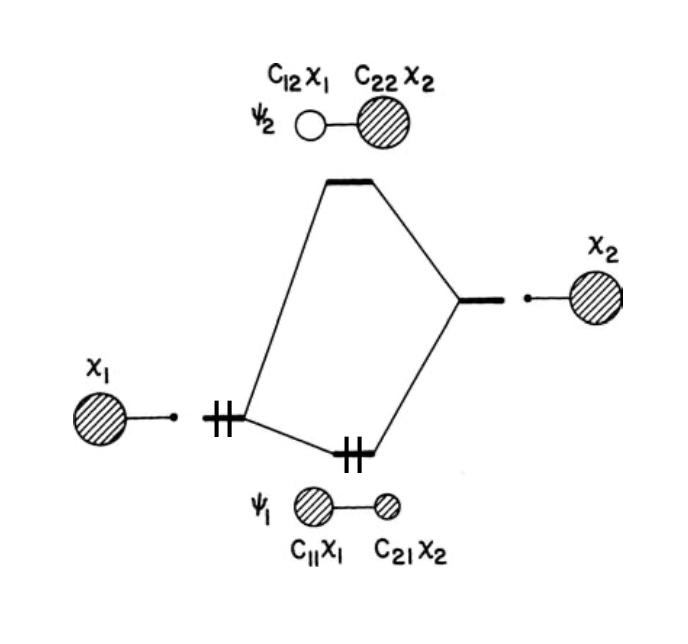
\includegraphics{F_charge_transfer.png}
    \caption{Orbital diagram in the case of charge transfer interaction}
    \label{F:charge_transfer}
\end{figure}



\end{document}

\documentclass{article}
\usepackage{amssymb, amsmath, amsthm}
\usepackage[margin=1in]{geometry}
\usepackage{verbatim}
\usepackage{graphicx}
\usepackage{hyperref} % \url \href
\usepackage{docmute}

\newtheorem{definition}{Definition}
\newtheorem{theorem}{Theorem}
\newcommand{\heff}{\mathbb{H}^{\text{eff}}}
\newcommand{\pfrac}[2]{\frac{\partial #1}{\partial #2}}

\newcommand{\MO}{\textbf{MO}}
\newcommand{\AO}{\textbf{AO}}

\newcommand{\huptb}{\text{H}_0}
\newcommand{\order}[2]{#1^{(#2)}}
\newcommand{\statebra}[1]{\langle #1 |}
\newcommand{\stateket}[1]{| #1 \rangle}

\begin{document}

\section{Three Orbital Perturbation Problem}
We use a three orbital problem to illustrate the application of molecular orbital 
perturbation theory. We consider the problem given in figure \ref{F:three_orbital}
where the orbital energies are given in order 
$\varepsilon_{iA}^0 < \varepsilon_{kB}^0 <\varepsilon_{jA}^0$. We assume the unperturbed 
Hamiltonian and overlap matrix are diagonal in the basis $\psi_{iA}^0$, $\psi_{kB}^0$ and $\psi_{jA}^0$
and the perturbation is given by:
\begin{align}
    \delta S = \left(\begin{matrix}
        0 & 0 & \tilde{S}_{ij} \\
        0 & 0 & \tilde{S}_{kj} \\
        \tilde{S}_{ji} & \tilde{S}_{jk} & 0 
    \end{matrix}\right) ; \quad \delta H \propto - \delta S
\end{align}
where we used relationship $H_{\mu\nu} \propto (H_{\mu\mu} + H_{\nu\nu}) S_{\mu\nu} $
and $H_{ii} < 0$ (because of the nature of ion-electron interaction). 

\begin{figure}[h!]
    \centering
    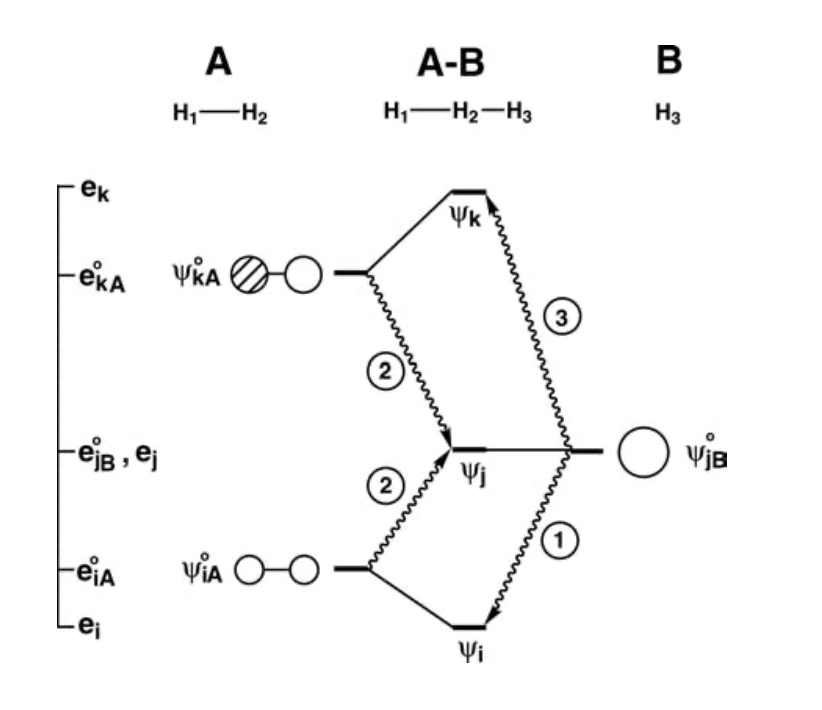
\includegraphics[width=4in]{three_orbital.png}
    \caption{Molecular Orbital diagram for the three orbital problem}
    \label{F:three_orbital}
\end{figure}

We use the perturbation theory result to obtain the approximate shape of the perturbed 
wavefunctions. We first focus on perturbed orbital $\psi_{i}$ derived from $\psi_{iA}$, 
using the assumed form of perturbation matrix, up to second order.
\begin{align}
    \psi_{i} &= 
    \left[ 1 -  \frac{(\tilde{H}_{ij} - \order{\varepsilon_i}{0}\tilde{S}_{ij})\tilde{S}_{ij}}{\order{\varepsilon_i}{0} - \order{\varepsilon_j}{0}} \right.
    \left. - \frac{1}{2} \left(\frac{\tilde{H}_{ij} - \order{\varepsilon_i}{0}\tilde{S}_{ij}}{\order{\varepsilon_i}{0} - \order{\varepsilon_j}{0}} \right)^2 \right] \psi_{iA}^0 \\ 
    &+ \left[ \frac{\tilde{H}_{ij}- \order{\varepsilon_i}{0} \tilde{S}_{ij}}{\order{\varepsilon_i}{0} - \order{\varepsilon_j}{0}} \right.
    + \left. \frac{(\tilde{H}_{ik}- \order{\varepsilon_i}{0} \tilde{S}_{ik})(\tilde{H}_{kj}- \order{\varepsilon_i}{0} \tilde{S}_{kj})}{(\order{\varepsilon_i}{0} - \order{\varepsilon_j}{0})(\order{\varepsilon_i}{0} - \order{\varepsilon_k}{0})} \right] \psi_{jB}^0  \\
    &+ \left[ \frac{\tilde{H}_{ik}- \order{\varepsilon_i}{0} \tilde{S}_{ik}}{\order{\varepsilon_i}{0} - \order{\varepsilon_k}{0}} \right.
    + \left. \frac{(\tilde{H}_{ij}- \order{\varepsilon_i}{0} \tilde{S}_{ij})(\tilde{H}_{jk}- \order{\varepsilon_i}{0} \tilde{S}_{jk})}{(\order{\varepsilon_i}{0} - \order{\varepsilon_k}{0})(\order{\varepsilon_i}{0} - \order{\varepsilon_j}{0})} \right] \psi_{kA}^0 
\end{align}
We further note that the second term in the bracket for $\psi_{jB}^0$ and the first term in the bracket for $\psi_{kA}^0$ vanish due to $\tilde{S}_{ik} = \tilde{H}_{ik} = 0$
so that the result can be reduced to 
\begin{align}
    \psi_{i} &= 
    \left[ 1 -  \frac{(\tilde{H}_{ij} - \order{\varepsilon_i}{0}\tilde{S}_{ij})\tilde{S}_{ij}}{\order{\varepsilon_i}{0} - \order{\varepsilon_j}{0}} \right.
    \left. - \frac{1}{2} \left(\frac{\tilde{H}_{ij} - \order{\varepsilon_i}{0}\tilde{S}_{ij}}{\order{\varepsilon_i}{0} - \order{\varepsilon_j}{0}} \right)^2 \right] \psi_{iA}^0 \\ 
    &+ \left[ \frac{\tilde{H}_{ij}- \order{\varepsilon_i}{0} \tilde{S}_{ij}}{\order{\varepsilon_i}{0} - \order{\varepsilon_j}{0}} \right] \psi_{jB}^0 
    + \left[ \frac{(\tilde{H}_{ij}- \order{\varepsilon_i}{0} \tilde{S}_{ij})(\tilde{H}_{jk}- \order{\varepsilon_i}{0} \tilde{S}_{jk})}{(\order{\varepsilon_i}{0} - \order{\varepsilon_k}{0})(\order{\varepsilon_i}{0} - \order{\varepsilon_j}{0})} \right] \psi_{kA}^0 \\
    &= (1 + \order{t_{ii}}{2}) \psi_{iA}^0 + \order{t_{ji}}{1} \psi_{jB}^0 + \order{t_{ki}}{2}\psi_{kA}^0
\end{align}

Let's consider the sign of these mixing coefficients, it can be seem that they mostly depend on the sign of the overlap integral $S_{ij}$ as well as the relative 
energy level between the orbitals. In the case of figure \ref{F:three_orbital}, we find the parameters:
\begin{equation}
    \tilde{S}_{ij}, \tilde{S}_{kj} > 0 
\end{equation}
and take $H_{\mu\nu} \propto (H_{\mu\mu} + H_{\nu\nu}) S_{\mu\nu} \propto - S_{\mu\nu}$ as well as $(H_{\mu\nu} - \varepsilon^0 S_{\mu\nu}) \propto - S_{\mu\nu} $
since the second term is relatively small. Now, we can determine the sign of the mixing coefficients:
\begin{align}
    \order{t_{ii}}{2} &= - [ (+) + (+) ] < 0 \\ 
    \order{t_{ji}}{1} &= \frac{(-)}{(-)} > 0 \\
    \order{t_{ki}}{2} &= \frac{(+)}{(+)} > 0
\end{align}
So that we find that both $\psi_{jB}^0$ and $\psi_{kA}^0$ mix positively into $\psi_{iA}^0$ in first order and second order. The obtained orbital 
can be approximately shown as in figure \ref{F:psi_i}. 
\begin{figure}[h!]
    \centering
    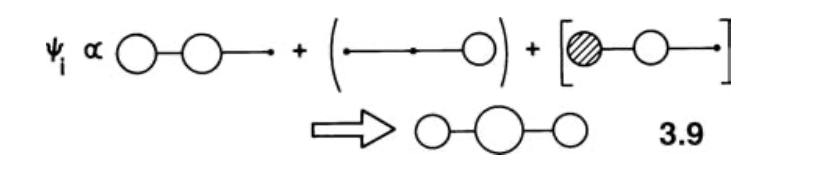
\includegraphics[width=4in]{psi_i.png}
    \caption{Orbital $\psi_{i}$}
    \label{F:psi_i}
\end{figure}

At this point, it is possible to point out a simple rule related to the sign of mixing coefficient 
for first order interaction, since it is simply given by the formula:
\[ t_{ji}^{(1)} = \frac{\tilde{H}_{ij}- \order{\varepsilon_i}{0} \tilde{S}_{ij}}{\order{\varepsilon_i}{0} - \order{\varepsilon_j}{0}}\] 
suppose that the orbitals are aligned so that $\tilde{S}_{ij}$ when they are brought together, we can 
see that:
\begin{itemize}
    \item The higher energies orbital mix \emph{into} the lower energy orbital with positive coefficients and,
    \item The lower energies orbital is substracted from the higher energy orbitals with a negative coefficients.
\end{itemize}

The other two orbitals can be obtained in the same fashion. The results are listed as follows:
\begin{align}
    \psi_{j} \approx \psi_{jB}^0 + |\order{t_{ij}}{1}| \psi_{iA}^0 - |\order{t_{kj}}{1}| \psi_{kA}^0 \\ 
    \psi_k \approx \psi_{kA}^0 - |\order{t_{jk}}{1}| \psi_{jB}^0 + |\order{t_{ik}}{2}| \psi_{iA}^0
\end{align}
where the sign correspond to the sign of the mixing coefficient $t$. The orbital are illustrated in figure \ref{F:psi_jk}.
\begin{figure}[h!]
    \centering
    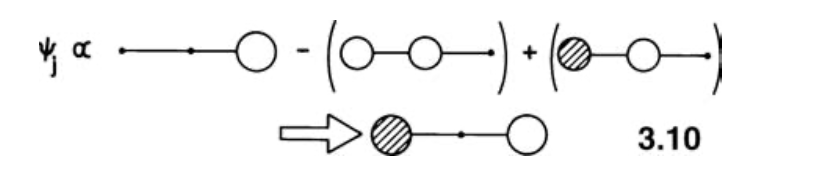
\includegraphics[width=4in]{psi_j.png}
    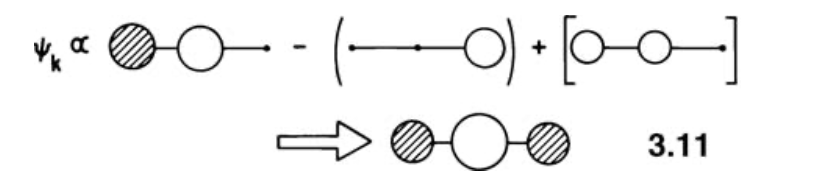
\includegraphics[width=4in]{psi_k.png}
    \caption{Orbital $\psi_{i}$ and $\psi_{k}$}
    \label{F:psi_jk}
\end{figure}


\end{document}

\documentclass{article}

\usepackage{amssymb, amsmath, amsthm}
\usepackage[margin=1in]{geometry}
\usepackage{verbatim}
\usepackage{graphicx}
\usepackage{hyperref} % \url \href
\usepackage{docmute}
\usepackage[title]{appendix}

\newtheorem{definition}{Definition}
\newtheorem{theorem}{Theorem}
\newcommand{\heff}{\mathbb{H}^{\text{eff}}}
\newcommand{\pfrac}[2]{\frac{\partial #1}{\partial #2}}
\newcommand{\huptb}{\text{H}_0}
\newcommand{\order}[2]{#1^{(#2)}}
\newcommand{\statebra}[1]{\langle #1 |}
\newcommand{\stateket}[1]{| #1 \rangle}
\newcommand{\MO}{\textbf{MO}}
\newcommand{\AO}{\textbf{AO}}

\begin{document}

\section{Symmetry Consideration}
The detailed treatment of symmetry consideration can be found in other books. Here I only
collect some notation and points important for our purpose. 
\subsection{Notation for Irreducible representation}
The notation for irreducible representation are usually used as follows:
\begin{enumerate}
    \item $A$ singly degenerate, symmetrical with respect to rotation about the principle axis (characters of these rotation are 1)
    \item $B$ singly degenerate, but antisymmetrical with repect to rotation about the principle axis (characters of these rotation are -1)
    \item $E$ doubly and $T$ triply degenerate representations.
    \item If there are more than one representation with the same label, we can use subscript: $A_1$, $A_2$ and so on.
    \item The representation with $\chi(i) = 1$ (symmetry under inversion) are given subscript $g$ (German \emph{gerade} = even)
    \item The representation that is antisymmetrical under inversion are given subscript $u$ (\emph{ungerade})
    \item The representation that is symmetrical with respect to $\sigma_h$ ($\chi(\sigma_h) = 1$) are given $'$, the representation 
            that is antisymmetrical with respect to $\sigma_h$ are given $''$ superscript.
\end{enumerate}
For a full description of the symbol, refer to \emph{Point Group Theory Table, Altmann, 1994, Page 63}. 
Usually, uppercase characters for the representation are used to denote electronic states. For 
atomic and molecular orbitals, as well as molecular vibrations, lowercase notation is used, e.g. 
$a_1, e, t_g$.

\subsection{Symmetry Consideration in Integrals} 
Symmetry require all integrals of the overlap $\statebra{\psi_a} \psi_b \rangle$ or 
interaction $\statebra{\psi_a} H \stateket{\psi_b}$ to vanish unless the wavefunction
$\stateket{\psi_a}$ and $\stateket{\psi_b}$ transform as the same irreducible 
representation of the molecular point group. Therefore, only the orbitals of the 
same symmetry may interact with each other. 

\subsection{Symmetry and Molecular Orbital Perturbation}
Let's consider the use of symmetry in the problem of molecular orbital perturbation. 
The main point here is the use of symmetry adapted molecular orbitals as the 
unperturbed states which reduce the number of interaction terms to consider in 
orbital mixing. Consider a diatomic molecular with $s$ and $p$ orbitals 
on each of the atoms and let's assume that in the begining, their interatomic 
separation is large so that the two atoms do not affect each other but then 
they are brought closer to form a molecular. We note in this case, the symmetry 
of the molecular do not change, so it is possible to form the symmetry adapted 
MOs as they are brought closer (interaction is turned on). For the total 8 orbitals, we 
focus on the $p_z$ orbitals as well as $s$ orbitals because interactions are allowed 
between them. They form 4 SALCs, with suitable normalization factor:
\begin{align*}
    \psi_1^{\sigma_u} &= \chi_s^1 - \chi_s^2 \\ 
    \psi_2^{\sigma_g} &= \chi_s^1 + \chi_s^2 \\ 
    \psi_3^{\sigma_u} &= \chi_{p_z}^1 + \chi_{p_z}^2 \\ 
    \psi_4^{\sigma_g} &= \chi_{p_z}^1 - \chi_{p_z}^2 
\end{align*}
where the superscript on $\chi$ indicate from which atom the wavefunction came. 
The unperturbed Hamiltonian contain degenerate energy of the $s$ ($\varepsilon_s$) 
and $p$ ($\varepsilon_p$) orbitals 
themselves of isolated atoms, and the perturbation is given by:
\begin{equation}
    \delta S = \left(\begin{matrix}
        \tilde{S}_{11} & 0 & \tilde{S}_{13} & 0 \\ 
        0 & \tilde{S}_{22} & 0 & \tilde{S}_{24} \\ 
        \tilde{S}_{31} & 0 & \tilde{S}_{33} & 0 \\ 
        0 & \tilde{S}_{42} & 0 & \tilde{S}_{44}
    \end{matrix}\right); \qquad
    \delta H = \left(\begin{matrix}
        \tilde{H}_{11} & 0 & \tilde{H}_{13} & 0 \\ 
        0 & \tilde{H}_{22} & 0 & \tilde{H}_{24} \\ 
        \tilde{H}_{31} & 0 & \tilde{H}_{33} & 0 \\ 
        0 & \tilde{H}_{42} & 0 & \tilde{H}_{44}
    \end{matrix}\right) \propto - \delta S
\end{equation}
It is noted that the diagonal elements of the perturbation in the overlap matrix 
$\delta H$ is now non-zero because the orbitals are distributed on different atoms 
that are brought closer. Their signs are given as:
$\tilde{S}_{11} < 0$, 
$\tilde{S}_{22} > 0$, 
$\tilde{S}_{33} < 0$, 
$\tilde{S}_{44} > 0$, 
$\tilde{S}_{13} < 0$ and 
$\tilde{S}_{24} > 0$. For the sign of $\delta H$, we can simply take the negative 
of $\delta H$. The first order correction in energies as the atoms are brought together 
is simply given by the diagonal elements: 
$(\tilde{H}_{ii} - \order{\varepsilon_i}{0} \tilde{S}_{ii})$. With first order correction, 
we can obtain the following energy diagram shown in figure \ref{F:A2_first_order}.
\begin{figure}[h!]
    \centering
    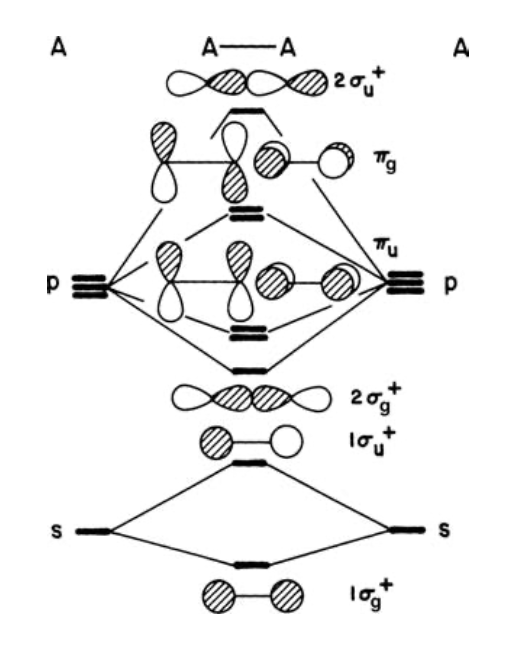
\includegraphics[width=2in]{F_A2_first_order.png}
    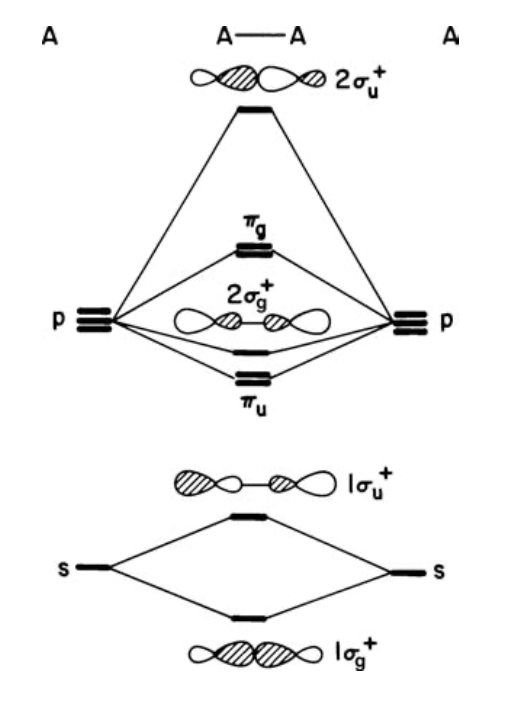
\includegraphics[width=3in]{F_A2_second_order.png}
    \caption{Left: First order correction for a diatomic moleculars and 
             right: First order correction to the wavefunction and second order correction to the energies}
    \label{F:A2_first_order}
\end{figure}

Let's now consider the first order correction to the wavefunctions and the resulting 
second order change in energies. We find:
\begin{align}
    \psi_1' \approx  \psi_1^{\sigma_u} + \frac{\tilde{H}_{13} - \varepsilon_s \tilde{S}_{13}}{\varepsilon_s - \varepsilon_p} \psi_3^{\sigma_u} 
            \approx \psi_1^{\sigma_u} - |\order{t_{31}}{1}| \psi_3^{\sigma_u} \\ 
    \psi_3' \approx  \psi_3^{\sigma_u} + \frac{\tilde{H}_{13} - \varepsilon_p \tilde{S}_{13}}{\varepsilon_p - \varepsilon_s} \psi_1^{\sigma_u}
            \approx \psi_3^{\sigma_u} + |\order{t_{13}}{1}| \psi_1^{\sigma_u} \\ 
    \psi_2' \approx  \psi_2^{\sigma_g} + \frac{\tilde{H}_{24} - \varepsilon_s \tilde{S}_{24}}{\varepsilon_s - \varepsilon_p} \psi_4^{\sigma_g} 
            \approx \psi_2^{\sigma_u} + |\order{t_{42}}{1}| \psi_4^{\sigma_g} \\ 
    \psi_4' \approx  \psi_4^{\sigma_g} + \frac{\tilde{H}_{24} - \varepsilon_p \tilde{S}_{24}}{\varepsilon_p - \varepsilon_s} \psi_2^{\sigma_g} 
            \approx \psi_4^{\sigma_u} - |\order{t_{24}}{1}| \psi_2^{\sigma_g}
\end{align}
since $\tilde{S}_{24} > 0$, the higher energy orbital $\psi_4$ mix into the lower energy orbitals $\psi_2$ and vice versa. Furthermore, we note 
that since orbitals can only mix if they have the same symmetry, the resulting orbitals also have the same symmetry. With the 
corrected wavefunctions, the energy corrections up to second order can be obtained. 
The resulting orbital diagram can be plotted as in figure \ref{F:A2_first_order} on the right. 


\end{document}

\documentclass{article}
\usepackage{amssymb, amsmath, amsthm}
\usepackage[margin=1in]{geometry}
\usepackage{verbatim}
\usepackage{graphicx}
\usepackage{hyperref} % \url \href
\usepackage{docmute}

\newtheorem{definition}{Definition}
\newtheorem{theorem}{Theorem}
\newcommand{\heff}{\mathbb{H}^{\text{eff}}}
\newcommand{\pfrac}[2]{\frac{\partial #1}{\partial #2}}

\newcommand{\MO}{\textbf{MO}}
\newcommand{\AO}{\textbf{AO}}

\newcommand{\huptb}{\text{H}_0}
\newcommand{\order}[2]{#1^{(#2)}}
\newcommand{\statebra}[1]{\langle #1 |}
\newcommand{\stateket}[1]{| #1 \rangle}

\begin{document}

\section{Electronegative and Geometric Perturbations}
\subsection{Electronegative Perturbation}
The benefit of performing perturbation calculation is that we can first tackle 
problems with the highest symmetry possible so as to utilize symmetry to the most,
and then choose the desired approximation methods to give a more accurate 
solution. Let's first consider the case of electronegative perturbation. For simplicity, 
we consider the two orbital problem for $s$ orbitals on a diatomic molecular. This 
example also illustrates the transformation of perturbation terms from MOs to AOs. 

Let's define the unperturbed molecular to be H$_2$ molecular, whose orbital diagonal we 
have already solved. Let's write:
\begin{align*}
    \psi_1 = a (s_1 + s_2) \\ 
    \psi_2 = b (s_1 - s_2)
\end{align*}
Because of the non-neglectable overlap between the two $s$ wavefunctions, coefficients $a$ and $b$
deviate from $\sqrt{2}/2$. 
This case correspond to our high symmetry case. Suppose now one of the 
H ion is replaced by a He ion and we further suppose its only effect is to introduce:
\begin{equation*}
    \statebra{s_2} H^{(\text{He})} \stateket{s_2} = \statebra{s_2} H^{(\text{H})} \stateket{s_2} + \delta v
\end{equation*}
since He ion is more electronegative than H, $\delta V < 0$. We assume here that the interaction 
terms $\statebra{s_1} \delta H \stateket{s_2} = 0$ and orbital $\stateket{s_1}$ is also not affected. The perturbation 
can be written in matrix form:
\begin{equation*}
    \delta H^{AO} = \left(\begin{matrix}
        0 & 0 \\ 0 & \delta v
    \end{matrix}\right), \qquad 
    \delta H^{MO} = \left(\begin{matrix}
        a^2 & -ab  \\ -ab  & b^2
    \end{matrix}\right) \delta v
\end{equation*}
where the relationship $H_{ij} = \sum_{\mu \nu} c_{\mu i} c_{\nu j} H_{\mu \nu}$ is used. With this we can solve 
the perturbed molecular orbitals to first order in wavefunction and second order correction in energy:
\begin{align*}
    \psi_1' \approx \psi_1 + \frac{\tilde{H}_{12}}{\varepsilon_1 - \varepsilon_2} \psi_2 \approx \psi_1 - |t_{21}| \psi_2 \\ 
    \psi_2' \approx \psi_2 + \frac{\tilde{H}_{12}}{\varepsilon_2 - \varepsilon_1} \psi_1 \approx \psi_2 + |t_{12}| \psi_1
\end{align*}
where $\tilde{H}_{12} = -ab\cdot \delta v > 0$, and the perturbated energies to second order is:
\begin{align*}
    \varepsilon_1' = \varepsilon_1 + a^2 \cdot \delta v + \frac{(-ab\cdot \delta v)^2}{\varepsilon_1 - \varepsilon_2} \\ 
    \varepsilon_2' = \varepsilon_2 + b^2 \cdot \delta v + \frac{(-ab\cdot \delta v)^2}{\varepsilon_2 - \varepsilon_1} 
\end{align*}
We note that energy correction to first order are negative for both terms, since introducing a more electronegative ion 
lower the energies of the system in total. The sign of second order perturbation is however different.

\subsection{Geometry Perturbation}
When the geometry of the molecular is distorted, the perturbation in terms of molecular orbitals can found as:
\begin{align}
    \tilde{H}_{ij} &= \sum_{\mu}\sum_{\nu} c_{\mu i}^0 \delta H_{\mu \nu} c_{\nu j}^0 \\ 
    \tilde{S}_{ij} &= \sum_{\mu}\sum_{\nu} c_{\mu i}^0 \delta S_{\mu \nu} c_{\nu j}^0 
\end{align} 
If the two geometries under consideration are similar, we should have $\delta S_{\mu \nu} \to 0$. Still, the relationship
$\delta H_{\mu \nu} \propto - \delta S_{\mu \nu}$ is largely true. An non-zero geometry perturbation will change most 
of the values of matrix elements $\delta H_{\mu \nu}$ and $\delta S_{\mu \nu}$. But starting from the perturbation 
matrix $\tilde{H}_{ij}$ and $\tilde{S}_{ij}$, we can treat the geometry perturbation using the perturbation formulism 
developed. We also note that with molecualr orbitals, the diagonal overlap matrix will also be nonzero with the 
MOs are distributed on different fragments of the distorted structure. For continuous geometric perturbation, energy 
levels can be organized into \emph{Walsh diagram}, such as shown in figure \ref{F:walsh_diagram}.
\begin{figure}[h!]
    \centering
    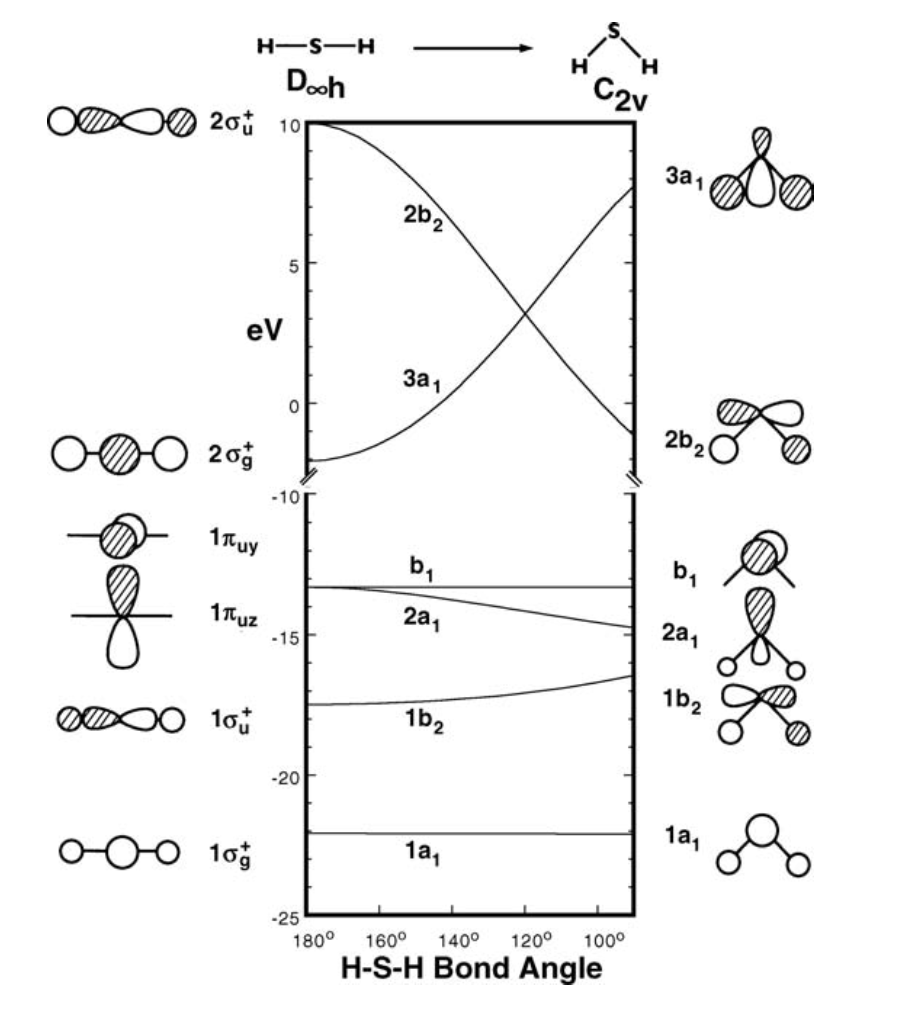
\includegraphics[width=3in]{F_walsh_diagram.png}
    \caption{Walsh diagram from a linear AH$_2$ to a trianglar AH$_2$}
    \label{F:walsh_diagram}
\end{figure}

\end{document}

\documentclass{article}
\usepackage{amssymb, amsmath, amsthm}
\usepackage[margin=1in]{geometry}
\usepackage{verbatim}
\usepackage{graphicx}
\usepackage{hyperref} % \url \href
\usepackage{docmute}

\newtheorem{definition}{Definition}
\newtheorem{theorem}{Theorem}
\newcommand{\heff}{\mathbb{H}^{\text{eff}}}
\newcommand{\pfrac}[2]{\frac{\partial #1}{\partial #2}}

\newcommand{\MO}{\textbf{MO}}
\newcommand{\AO}{\textbf{AO}}

\newcommand{\huptb}{\text{H}_0}
\newcommand{\order}[2]{#1^{(#2)}}
\newcommand{\statebra}[1]{\langle #1 |}
\newcommand{\stateket}[1]{| #1 \rangle}

\begin{document}

\section{Through-bond Interaction}
In this section, we provide example of how the presense of some bonds 
affect other bonds in molecular. As we can see, such bond-bond interaction 
can be understood following the consideration of molecular orbital 
perturbation treatment. 

\subsection{Bond-bond Interaction}
Let's consider the molecular orbital of C$_3$H$_6$ and its variant to illustrate the 
how the presense of orbitals change the interaction between other bonds and eventually the 
geometry of the molecular structure. First, let's construct the molecular orbital diagram 
of the C$_3$H$_6$ molecular itself. Instead of starting from the entire molecular, we first 
consider the MO diagram of the CH$_2$ fragments.  


\end{document}

\documentclass{article}
\usepackage{amssymb, amsmath, amsthm}
\usepackage[margin=1in]{geometry}
\usepackage{verbatim}
\usepackage{graphicx}
\usepackage{hyperref} % \url \href
\usepackage{docmute}

\newtheorem{definition}{Definition}
\newtheorem{theorem}{Theorem}
\newcommand{\heff}{\mathbb{H}^{\text{eff}}}
\newcommand{\pfrac}[2]{\frac{\partial #1}{\partial #2}}

\newcommand{\MO}{\textbf{MO}}
\newcommand{\AO}{\textbf{AO}}

\newcommand{\huptb}{\text{H}_0}
\newcommand{\order}[2]{#1^{(#2)}}
\newcommand{\statebra}[1]{\langle #1 |}
\newcommand{\stateket}[1]{| #1 \rangle}

\begin{document}

\section{Molecular Orbitals in Conjugated System and Solids}
\subsection{Conjugated System}
Conjugated system\footnote{\url{https://en.wikipedia.org/wiki/Conjugated_system}} 
refer to systems consists of connected $p$ orbitals with delocalized electrons in a molecular. 
Let's consider $N$ $\pi$ orbitals along a chain with nearest neighbor interaction and 
we further assume that their orbitals are non-overlapping so that the matrix 
element is $S_{\mu\nu} = \delta_{\mu\nu}$. 
The reason that we choose $\pi$ orbital system is because the small orbital overlap in this 
situation, as compared to the head to head sigma interactions. 
Let the energy of the $p$ orbital itself to be $\alpha$
and the nearest neighbor interaction $\beta < 0$, the secular equation can be reduced to 
an eigen-equation:
\begin{equation}
    H^{AO} \mathbf{C}_i = \varepsilon_i \mathbf{C}_i
\end{equation}
where the form of the Hamiltonian is like:
\begin{equation}
    H^{AO}_{N=3} = \left(\begin{matrix}
        \alpha & \beta & 0 \\ 
        \beta & \alpha & \beta \\ 
        0 & \beta & \alpha 
    \end{matrix}\right)
\end{equation}
The solution of the eigen-equation is given by:
\begin{align}
    \varepsilon_j &= \alpha + 2 \beta \cos\frac{j\pi}{N+1} \\ 
    c_{\mu j} &= \left(\frac{2}{N+1}\right)^{1/2} \sin\left(\frac{\mu j\pi}{N+1}\right) 
\end{align}
where $j$ index\footnote{$j$ is used instead of $i$ to avoid confusion with imaginary number $i$} 
the obtained molecular orbital and $\mu$ index the consistuting atomic orbitals. 

The importance of the factor $N+1$ can be shown as follows: we subsitute the solution into the 
eigen-equation:
\begin{equation}
    \sum_{\nu} H_{\mu\nu} C_{\nu j} = H_{\mu\mu-1} C_{\mu-1 j} + H_{\mu\mu} C_{\mu j} + H_{\mu\mu+1} C_{\mu+1 j} = \varepsilon_j C_{\mu j}
\end{equation}
where we use the fact that the summation is restricted to the nearest neighbors only. Using the 
solution, we obtain the expression:
\begin{align}
    &\left(\alpha + 2 \beta \cos\frac{j\pi}{N+1}\right) \sin\frac{\mu j\pi}{N+1} \\
    &= \alpha \sin\frac{\mu j\pi}{N+1} + 2 \beta \cos\frac{j\pi}{N+1} \sin\frac{\mu j\pi}{N+1} \\ 
    &= \left[\beta\cdot \sin\frac{(\mu-1) j\pi}{N+1}  \right. 
     \left. + \alpha\cdot\sin\frac{\mu j\pi}{N+1}  + \beta \cdot \sin \frac{(\mu+1) j\pi}{N+1}\right] 
\end{align} 
where the common normalization factor $(2/(N+1))^{1/2}$ is removed. The term with $\alpha$ are the same on both side 
so we only need to show that:
\begin{equation}
    2 \beta \cos\frac{j\pi}{N+1} \sin\frac{\mu j\pi}{N+1} 
    = \beta\cdot \sin\left( \frac{\mu j\pi}{N+1} - \frac{j\pi}{N+1} \right) 
    + \beta\cdot \sin\left( \frac{\mu j\pi}{N+1} + \frac{j\pi}{N+1} \right)
\end{equation}
For $1 \leq \mu \leq N$. We can consider three cases: 
For $\mu = 1$, the right hand side become:
\begin{equation}
    \beta\cdot \sin\left( \frac{j\pi}{N+1} + \frac{j\pi}{N+1} \right) 
    = 2 \beta \sin \frac{j\pi}{N+1} \cos \frac{j\pi}{N+1} 
\end{equation}
since $\sin(2\alpha) = 2\sin\alpha\cos\alpha$. 
For $1 < \mu < N$, we can similarly show that the equality is true with 
$\sin(\alpha \pm \beta) = \sin\alpha\cos\beta \pm \sin\beta\cos\alpha$. 
The effect of factor $N+1$ is shown when $\mu = N$, in which case we have, for the right hand side:
\begin{align}
    \beta\cdot \sin\left( \frac{N j\pi}{N+1} - \frac{j\pi}{N+1} \right) 
    &= \beta \left( \sin\frac{N j\pi}{N+1}\cos\frac{j\pi}{N+1} - \cos\frac{N j\pi}{N+1}\sin\frac{j\pi}{N+1}  \right) \\ 
    &= \beta \left( \sin\frac{N j\pi}{N+1}\cos\frac{j\pi}{N+1} - \cos\left(1 - \frac{j\pi}{N+1}\right)\sin\left(1 - \frac{Nj\pi}{N+1}\right)  \right) \\ 
    &=2 \beta \sin\frac{N j\pi}{N+1}\cos\frac{j\pi}{N+1}
\end{align}
If we have $N$ instead of $N+1$, then the last situation will not be correct.

\subsection{Cyclic systems}
Let's now consider the case of cyclic system with single $s$ orbitals on each site and nearest neighbor interaction. 
This situation is close to that in solids with periodic boundary condition. The solution is now given by:
\begin{align}
    \label{E:cyclic_system_energy}
    \varepsilon_j &= \alpha + 2 \beta \cos\frac{j\pi}{N} \\ 
    c_{\mu j} &= \frac{1}{\sqrt{N}} \exp \frac{2\pi i \cdot j (\mu-1)}{N} 
\end{align}
where we take the index of $j$ to start from 0. 
The energy level obtained in such approach can be graphically shown as in figure \ref{F:cyclic_energy} 
where we can always find a single degenerate state at energy $\alpha + 2 \beta$. If $N$ is even, we have 
another single degenerate state with energy $\alpha - 2 \beta$. All the other states are doubly degenerate. 
\begin{figure}[h!]
    \centering
    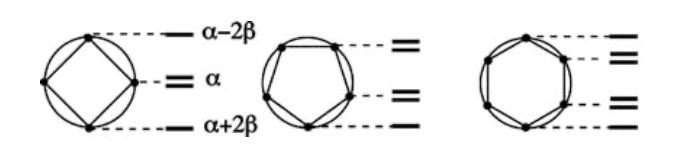
\includegraphics[width=3in]{F_cyclic_energy.png}
    \caption{Graphical illustration of cyclic energy}
    \label{F:cyclic_energy}
\end{figure}
This is true for cyclic groups $C_n$ if we check their character tables, as shown for group $C_4$, $C_5$ and 
$C_6$ in figure \ref{F_cyclic_group_table}

\begin{figure}[h!]
    \centering
    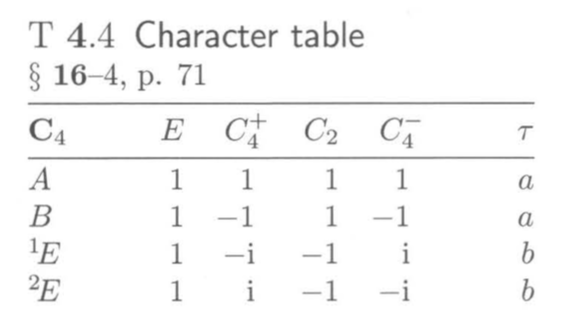
\includegraphics[width=3in]{F_C4.png}
    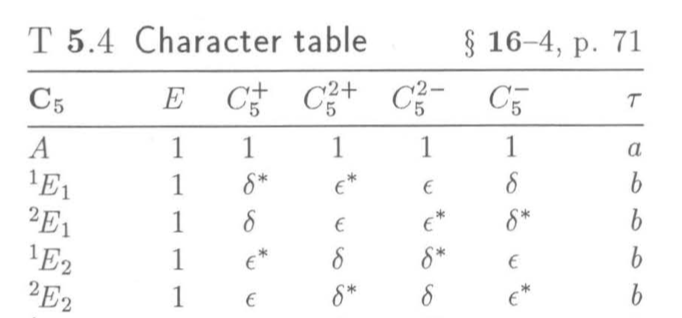
\includegraphics[width=3in]{F_C5.png}
    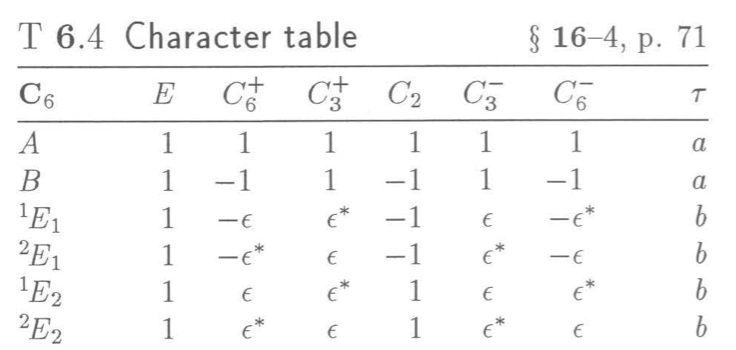
\includegraphics[width=3in]{F_C6.png}
    \caption{Character tables for cyclic groups}
    \label{F_cyclic_group_table}
\end{figure}

\subsection{Solids}
Let's consider as example, only the one dimension chain that extend infinitely in one direction but are joined 
at the two end, so that the situation is similar to that of the cyclic system. 
We use the interaction parameter similar to that of the cyclic system so that the energy can still be 
expressed using equation \eqref{E:cyclic_system_energy}. However, we use the vector $k$:
\begin{equation}
    k = \frac{2\pi j}{Na}
\end{equation}
so that the energy and wavefunction can be expressed as:
\begin{align}
    \varepsilon_j &= \alpha + 2 \beta \cos ka \\ 
    c_{\mu j} &= \frac{1}{\sqrt{N}} e^{ik(\mu-1) a} = \frac{1}{\sqrt{N}} e^{ikR_{\mu}}
\end{align}
where now each wavefunction $\chi_{\mu}$ is a considered to be in the $\mu$th cell. 

Let's now take into account the overlap matrix $S$. The eigenstates in solids are given 
by functions that satisfy the bloch condition: $\phi_k(r+l) = e^{ikl} \phi_k(r)$ where $l$ 
is a lattice vector. 
\begin{align}
    \psi_j^k(r) &= \sum_{\mu}c^k_{\mu j}\phi_{\mu}^k(r) \\ 
    \phi_{\mu}^k(r) &= \frac{1}{\sqrt{N}} \sum_p e^{ikR_p} \chi_{\mu}(r - R_p)
\end{align}
we can verify:
\begin{align}
    \psi_j^k(r+l) &= \frac{1}{\sqrt{N}} \sum_{\mu} c^k_{\mu j} \sum_p e^{ikR_p} \chi_{\mu}(r - (R_p - l)) \\ 
    &= \frac{1}{\sqrt{N}} \sum_{\mu} c^k_{\mu j} \sum_{p'} e^{ik(R_{p'}+l)} \chi_{\mu}(r - R_{p'}) \\ 
    &= e^{ikl} \phi_j^k(r)
\end{align}
Now, let's solve the eigenequation:
\begin{align}
    H \stateket{ \psi_j^k } &= \varepsilon_j^k \stateket{ \psi_j^k } \\ 
    \frac{1}{N} \sum_{\mu} c^k_{\mu j} \sum_{pp'} e^{ik(R_p - R_{p'})} \statebra{\chi_{\nu,R_{p'}}} H \stateket{\chi_{\mu,R_p}}
    &= \frac{1}{N}  \varepsilon_j^k \sum_{\mu} c^k_{\mu j} \sum_{pp'} e^{ik(R_p - R_{p'})} \statebra{\chi_{\nu,R_{p'}}} \chi_{\mu,R_p} \rangle \\ 
    \sum_{\mu} c^k_{\mu j} H_{\nu\mu}^k &= \varepsilon_j^k \sum_{\mu} c^k_{\mu j} S_{\nu\mu}^k \\ 
    \mathbf{H}^k \mathbf{C}_{j}^k &= \varepsilon_j^k \mathbf{H}^k \mathbf{S}_{j}^k
\end{align}
where we multiplied $\statebra{\phi_{\mu}^k}$ on the left for the second relationship. The final equation 
is the tight binding secular equation in solids, where 
\begin{align}
    H_{\nu\mu}^k = \sum_p e^{ikR_p} \statebra{\chi_{\nu,R_0}} H \stateket{\chi_{\mu,R_p}} \\ 
    S_{\nu\mu}^k = \sum_p e^{ikR_p} \statebra{\chi_{\nu,R_0}} \chi_{\mu,R_p} \rangle
\end{align}

\subsection{Interpretation of band dispersion with avoided crossing}
In this section, we point out the complication introduced by avoided crossing in 
Interpretation of band dispersion with a $sp$ one dimensional chain along $z$ direction 
with total 4 bands.
The case of $p_x$, $p_y$ and $s$ follows the above discussion. At the zone center, $k=0$ and we 
have the lowest energy $\varepsilon_{k=0} = \alpha + 2\beta$ and at the zone edge where $k = \pi/a$ 
we have the highest energy $\varepsilon_{k=\pi/a} = \alpha - 2\beta$. $\beta$ is defined to be a 
negative value. Therefore, these bands \emph{run up} in band dispersion along $\Gamma-X$. 
In terms of energy position, $p_x$ and $p_y$ bands are degenerate and located higher 
in energy compared to the $s$ bands. For $p_z$ band, its dispersion $runs down$, as can be 
seen from figure \ref{F:pz}. Furthermore, due to strong $\sigma$ interaction, the band is very dispersive. 

\begin{figure}[h!]
    \centering
    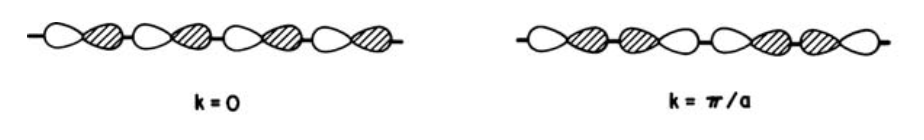
\includegraphics[width=3in]{F_pz.png}
    \caption{Wavefunction of the $p_z$ band at $k=0$ and $k=\pi/a$}
    \label{F:pz}
\end{figure}

It is clear that at both $k=0$ and $k=\pi/a$, these four bands cannot interact with each other 
because of the symmetry of the wavefunction: on each site the overlap integral vanish. However, 
this is not so on the path between $\Gamma$ and $X$ points. Along the line, $p_x$ and $p_y$ 
does not interact but $p_z$ and $s$ band does. Interaction created avoided crossing, as shown 
by the figure \ref{F:avoid_interaction}.

\begin{figure}[h!]
    \centering
    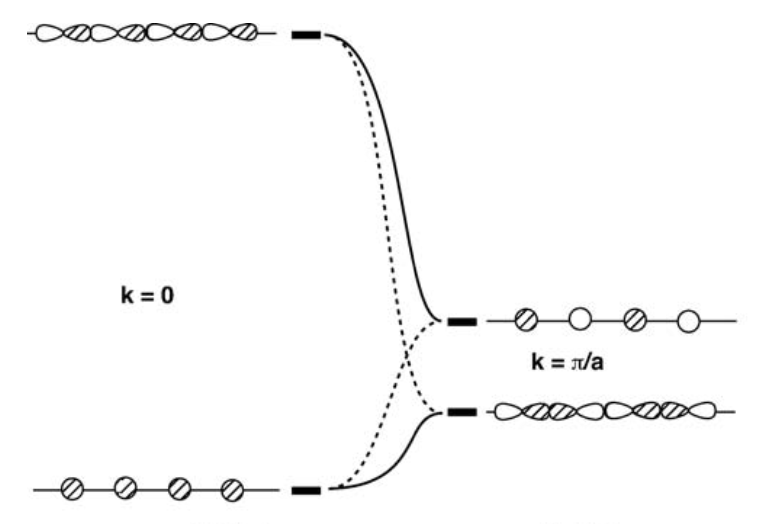
\includegraphics[width=2in]{F_avoid_interaction_spz.png}
    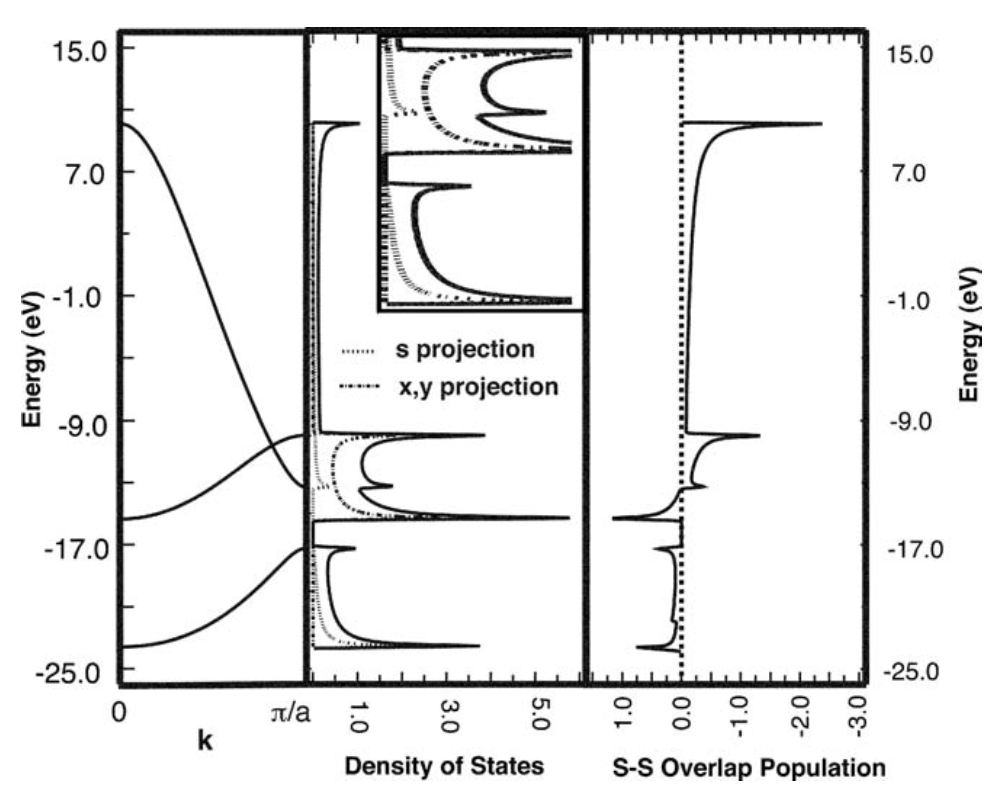
\includegraphics[width=3in]{F_avoid_interaction_dispersion.png}
    \caption{Avoid interaction in band dispersion}
    \label{F:avoid_interaction}
\end{figure}

It is now clear that although in the band dispersion, the $s$ band running up and $p_z$ band 
running down seems to be formed purely by $s$ and $p_z$ themselves, they are actually mixed. 
We use the lower $s$ band as an example for the consequence for the avoided crossing:
\begin{enumerate}
    \item Due to the mixing, the density of state of the upper part of the band is mainly $p_z$ character, and 
    \item Both the top and bottum of the band are $bonding$. This is opposite to the isolated case (for example $p_x$) where 
          the bottum of the band is bonding and the top are antibonding. 
\end{enumerate}

\end{document}

\documentclass{article}
\usepackage{amssymb, amsmath, amsthm}
\usepackage[margin=1in]{geometry}
\usepackage{verbatim}
\usepackage{graphicx}
\usepackage{hyperref} % \url \href
\usepackage{docmute}

\newtheorem{definition}{Definition}
\newtheorem{theorem}{Theorem}
\newcommand{\heff}{\mathbb{H}^{\text{eff}}}
\newcommand{\pfrac}[2]{\frac{\partial #1}{\partial #2}}

\newcommand{\MO}{\textbf{MO}}
\newcommand{\AO}{\textbf{AO}}

\newcommand{\huptb}{\text{H}_0}
\newcommand{\order}[2]{#1^{(#2)}}
\newcommand{\statebra}[1]{\langle #1 |}
\newcommand{\stateket}[1]{| #1 \rangle}

\begin{document}

\section{Spin Polarization}
\subsection{Many body states}
Multi-electron systems are fundamentally manybody problem, so single particle 
solutions are often not enough to present the true electronic structure of the 
system. We should have the following hierarchy:
\begin{enumerate}
    \item single particle states
    \item many-body hartree fock state using slater determinant
    \item mixture of hartree fock state
\end{enumerate}
Suppose that we have a set of orthogonal single particle states $\psi_i(r_{\mu})$, where $i$
index the single particle states and $r_{\mu}$ is the position of the $\mu$th particle. 
Spins are included in the wavefunction. Then a slater determinant is given as
\begin{equation}
    \Phi(r_1, \cdots, r_n) = \frac{1}{\sqrt{N!}} 
    \left| \begin{matrix}
        \psi_1(r_1) & \cdots & \psi_1(r_n) \\ 
        \psi_2(r_1) & \cdots & \psi_2(r_n) \\
        \vdots &  & \vdots \\ 
        \psi_n(r_1) & \cdots & \psi_n(r_n)
    \end{matrix} \right|
\end{equation}
which satisfy the antisymmetry under exchange of particle. 

Using these slater states as the initial ``unperturbed'' states, we can find their 
energy expectation values:
\begin{equation}
    E_{\Phi_a} = \statebra{\Phi_a(r_1, \cdots, r_n)} H \stateket{\Phi_a(r_1, \cdots, r_n)}
\end{equation}
Furthermore, the off-diagonal elements are also non-zero, leading to a treatment similar 
to the perturbation treatment. The true eigenstates can thus be written as a linear combination:
\begin{equation}
    \Psi_g = \sum_{i} c_{ig} \Phi_i
\end{equation}
by solving the Hamiltonian matrix with element $H_{ij} = \statebra{\Phi_i} H \stateket{\Phi_j}$. 

\subsection{Hartree Fock}


\subsection{Exchange Interaction and Spin polarization}


\end{document}


\begin{appendices}
    
% on the same page, section is numberd with A, B automatically
\documentclass{article}
\usepackage{amssymb, amsmath, amsthm}
\usepackage[margin=1in]{geometry}
\usepackage{verbatim}
\usepackage{graphicx}
\usepackage{hyperref} % \url \href
\usepackage{docmute}

\newtheorem{definition}{Definition}
\newtheorem{theorem}{Theorem}
\newcommand{\heff}{\mathbb{H}^{\text{eff}}}
\newcommand{\pfrac}[2]{\frac{\partial #1}{\partial #2}}

\begin{document}

\section{Another approach to obtain the Secular Equation}
Following the notation 
\begin{equation}
    \psi_i = \mathbf{\chi}\cdot \mathbf{C}_i = \sum_{\mu} C_{\mu i} \chi_{\mu}
\end{equation}
where the coefficients are assumed to be real and unknown. We denote:
\begin{align}
    H_{ij} &= \sum_{\mu\nu} c_{\mu i} c_{\nu i} H_{\mu \nu} \\ 
    S_{ij} &= \sum_{\mu\nu} c_{\mu i} c_{\nu i} S_{\mu \nu} 
\end{align}
let's seek to minimize the orbital energies:
\begin{equation}
    \varepsilon_i = \frac{\langle \psi_i | H | \psi_j \rangle}{\langle \psi_i | \psi_j \rangle} = \frac{B}{A}
\end{equation}
with respect to the coefficients $c_{\mu i}$:
\begin{equation}
    \pfrac{\varepsilon_i}{c_{\mu i}} = \pfrac{(B/A)}{c_{\mu i}} = \frac{1}{A} \pfrac{B}{c_{\mu i}} - \frac{B}{A^2} \pfrac{A}{c_{\mu i}} = 0
\end{equation}
The terms are given:
\begin{align}
    \pfrac{B}{c_{\mu i}} &= 2 \sum_{\nu} c_{\nu i} H_{\mu \nu} \\
    \pfrac{A}{c_{\mu i}} &= 2 \sum_{\nu} c_{\nu i} S_{\mu \nu} \\
\end{align}
so that we obtain the \emph{secular equation}:
\begin{equation}
    \label{E:secular}
    \sum_{\nu} \left[ H_{\mu\nu} - \varepsilon_i S_{\mu\nu} \right] c_{\nu i} = 0
\end{equation}

\end{document}

\documentclass{article}
\usepackage{amssymb, amsmath, amsthm}
\usepackage[margin=1in]{geometry}
\usepackage{verbatim}
\usepackage{graphicx}
\usepackage{hyperref} % \url \href
\usepackage{docmute}

\newtheorem{definition}{Definition}
\newtheorem{theorem}{Theorem}
\newcommand{\heff}{\mathbb{H}^{\text{eff}}}
\newcommand{\pfrac}[2]{\frac{\partial #1}{\partial #2}}

\newcommand{\huptb}{\text{H}_0}
\newcommand{\order}[2]{#1^{(#2)}}
\newcommand{\statebra}[1]{\langle #1 |}
\newcommand{\stateket}[1]{| #1 \rangle}

\begin{document}

\section{Perturbation Theory}
Suppose in the un-perturbed case, we have:
\begin{gather}
    \huptb \stateket{\order{n}{0}} = E_0 \stateket{\order{n}{0}} \quad \text{and} \quad
    \sum_n \stateket{\order{n}{0}}\statebra{\order{n}{0}} = 1
\end{gather}
and introduce perturbation $\text{H} = \huptb + \lambda V$ and solve the 
perturbed eigenequation:
\begin{equation}
    (\huptb + \lambda V) \stateket{n} = E \stateket{n}
\end{equation}
The parameter $\lambda$ switches on the perturbation and setting $\lambda = 1$ 
recovers the actual perturbed Hamiltonian. 
Introduce $\Delta_n = E_n - \order{E_n}{0}$, we 
can write:
\begin{align}
    (\huptb + \lambda V) \stateket{\order{n}{\lambda}} = (\Delta_n + \order{E_n}{0}) \stateket{\order{n}{\lambda}} \\
    (\huptb - \order{E_n}{0}) \stateket{\order{n}{\lambda}} = (\Delta_n - \lambda V) \stateket{\order{n}{\lambda}}
\end{align}
since $(\huptb - \order{E_n}{0})\stateket{\order{n}{0}} = 0$, we have:
\begin{equation}
    \label{E:result1}
    \statebra{\order{n}{0}} \Delta_n - \lambda V \stateket{n}
    = \statebra{\order{n}{0}} \huptb - \order{E_n}{0} \stateket{n} 
    = 0
\end{equation} 

Define a projection operator which exclude unperturbed states $|\order{n}{0}\langle$:
$\Phi_n = 1 - \stateket{\order{n}{0}}\statebra{\order{n}{0}} = \sum_{k\neq n} \stateket{\order{k}{0}}\statebra{\order{k}{0}}$. 
The projection operator commutes with the unperturbed Hamiltonian $\huptb$:
\begin{equation}
    ( 1 - \stateket{\order{n}{0}}\statebra{\order{n}{0}} ) \huptb
    = \huptb - \order{E_n}{0} \stateket{\order{n}{0}}\statebra{\order{n}{0}} 
    = \huptb ( 1 - \stateket{\order{n}{0}}\statebra{\order{n}{0}} )
\end{equation}
using the projection operator, we have:
\begin{equation}
    (\Delta_n - \lambda V) \stateket{n}
    = (\stateket{\order{n}{0}}\statebra{\order{n}{0}} + \Phi_n) (\Delta_n - \lambda V) \stateket{n} 
    = \Phi_n (\Delta_n - \lambda V) \stateket{n}
\end{equation}
On the other hand, we are free to add:
\begin{equation}
    (\huptb - \order{E_n}{0}) \stateket{n} = 
    (\huptb - \order{E_n}{0}) (-c\stateket{\order{n}{0}} + \stateket{n} )
\end{equation}
where $c$ is some arbitrary constants, gathering the results, we have equation:
\begin{gather}
    (\huptb - \order{E_n}{0}) (-c\stateket{\order{n}{0}} + \stateket{n} ) 
    = \Phi_n (\Delta_n - \lambda V) \stateket{n} \\
    \label{E:main2}
    \stateket{n} = \stateket{\order{n}{0}} 
    + \underbrace{\frac{1}{\huptb - \order{E_n}{0}} \Phi_n (\Delta_n - \lambda V) \stateket{n}}_{\text{orthogonal to } \stateket{\order{n}{0}}}
\end{gather}
where $c$ is set to $1$ so that 
when $\lambda = 0$, the second term will be zero since both $\Delta_n$ and $\lambda V$ are zero. 
At this moment, the perturbed states are not normalized. \eqref{E:main2}
We also note that the entire second term on the right hand side is orthogonal to state $\stateket{\order{n}{0}}$
because of the projection operator can also be written explicitly to be:
\begin{align}
    \frac{1}{\huptb - \order{E_n}{0}} \Phi_n (\Delta_n - \lambda V) \stateket{n}
    = \sum_{k\neq n} \ \frac{1}{\order{E_k}{0} - \order{E_n}{0}} \stateket{\order{k}{0}} \statebra{\order{k}{0}} (\Delta_n - \lambda V) \stateket{n}
\end{align}
Suppose we write $\stateket{n} = \stateket{\order{n}{0}} + \stateket{\delta  n}$, we find that equation
\eqref{E:result1} can be reduced to 
\begin{equation}
    \label{E:main1}
    \Delta_n = \statebra{\order{n}{0}} \lambda V \stateket{n}
\end{equation}
since $\statebra{\order{n}{0}} \Delta_n \stateket{\delta n} = 0$

Now, we write out the approximate expansion in orders of $\lambda$:
\begin{align}
    \Delta_n &= \lambda \order{\Delta_n}{1} + \lambda^2 \order{\Delta_n}{2} + \lambda^3 \order{\Delta_n}{3} + \cdots \\
    \stateket{n} &= \stateket{\order{n}{0}} + \lambda \stateket{\order{n}{1}} + 
                    \lambda^2 \stateket{\order{n}{2}} + \lambda^3 \stateket{\order{n}{3}} + \cdots
\end{align}
Substituting $\stateket{n}$ and $\Delta_n$ into equation \eqref{E:main1} and equating the terms in the same order,
we have the relationship:
\begin{gather}
    \order{\Delta_n}{1} = \statebra{\order{n}{0}} V \stateket{\order{n}{0}} \\
    \order{\Delta_n}{2} = \statebra{\order{n}{0}} V \stateket{\order{n}{1}} \\
    \cdots \\
    \order{\Delta_n}{i+1} = \statebra{\order{n}{0}} V \stateket{\order{n}{i}} \\
\end{gather}
Where we find that the $(i+1)$th perturbation energy depend on the $i$th perturbed states, 
now we can simply work up the order using equation \eqref{E:main2}:


\end{document}


\end{appendices}


\end{document}
